\section{High-level overview}

The goal of the translation is to model a Go program using GooseLang,
which is a programming language defined in Coq for this purpose. That is,
GooseLang is defined using expressions defined in Coq, equipped with a
semantics also given in Coq. \Cref{fig:goose:overview} gives a graphical
depiction of how Goose and GooseLang fit together. Since GooseLang programs support references
to model the Go heap, the semantics is written in terms of transitions
of (expression, heap) pairs where the heap maps pointers to values. The
intention of the translation is that the semantics of the translated
function should cover all the behaviors of the Go code, in terms of
return values and effect on the heap. As long as this is true, a proof
that the translated code always satisfies some specification means that
the real running code will, too.

GooseLang is a low-level language, so many constructs in Go translate to
(small) implementations in GooseLang. This implementation choice proved
to be much more convenient than adding primitives to the language for
every Go construct. For example, a slice is represented as a tuple of
pointer, length, and capacity, and appending to a slice requires
checking for available capacity and copying if none is available.
Appending to a slice is a complicated operation, and it was easier to
write it correctly as a program rather than directly as a transition in
the semantics. The one cost to this design strategy is that an arbitrary
GooseLang program is much more general than translated Go programs --- for
example, GooseLang has support for pointer arithmetic. This
has no impact on verifying any \emph{specific} Go program.

The extra generality of GooseLang is a downside when a theorem talks about an
\emph{arbitrary} GooseLang program, as shows up in the transaction system's
transaction refinement and simulation-transfer theorems. In order to make these
theorems true, they must rule out
some ill-defined GooseLang programs, which are
not possible to produce by writing Go and translating it to GooseLang. Both
specifications make these assumptions using a
standard technique of using a type system for GooseLang developed in Coq, and encoding
syntactic restrictions via that type system.

\begin{figure}
  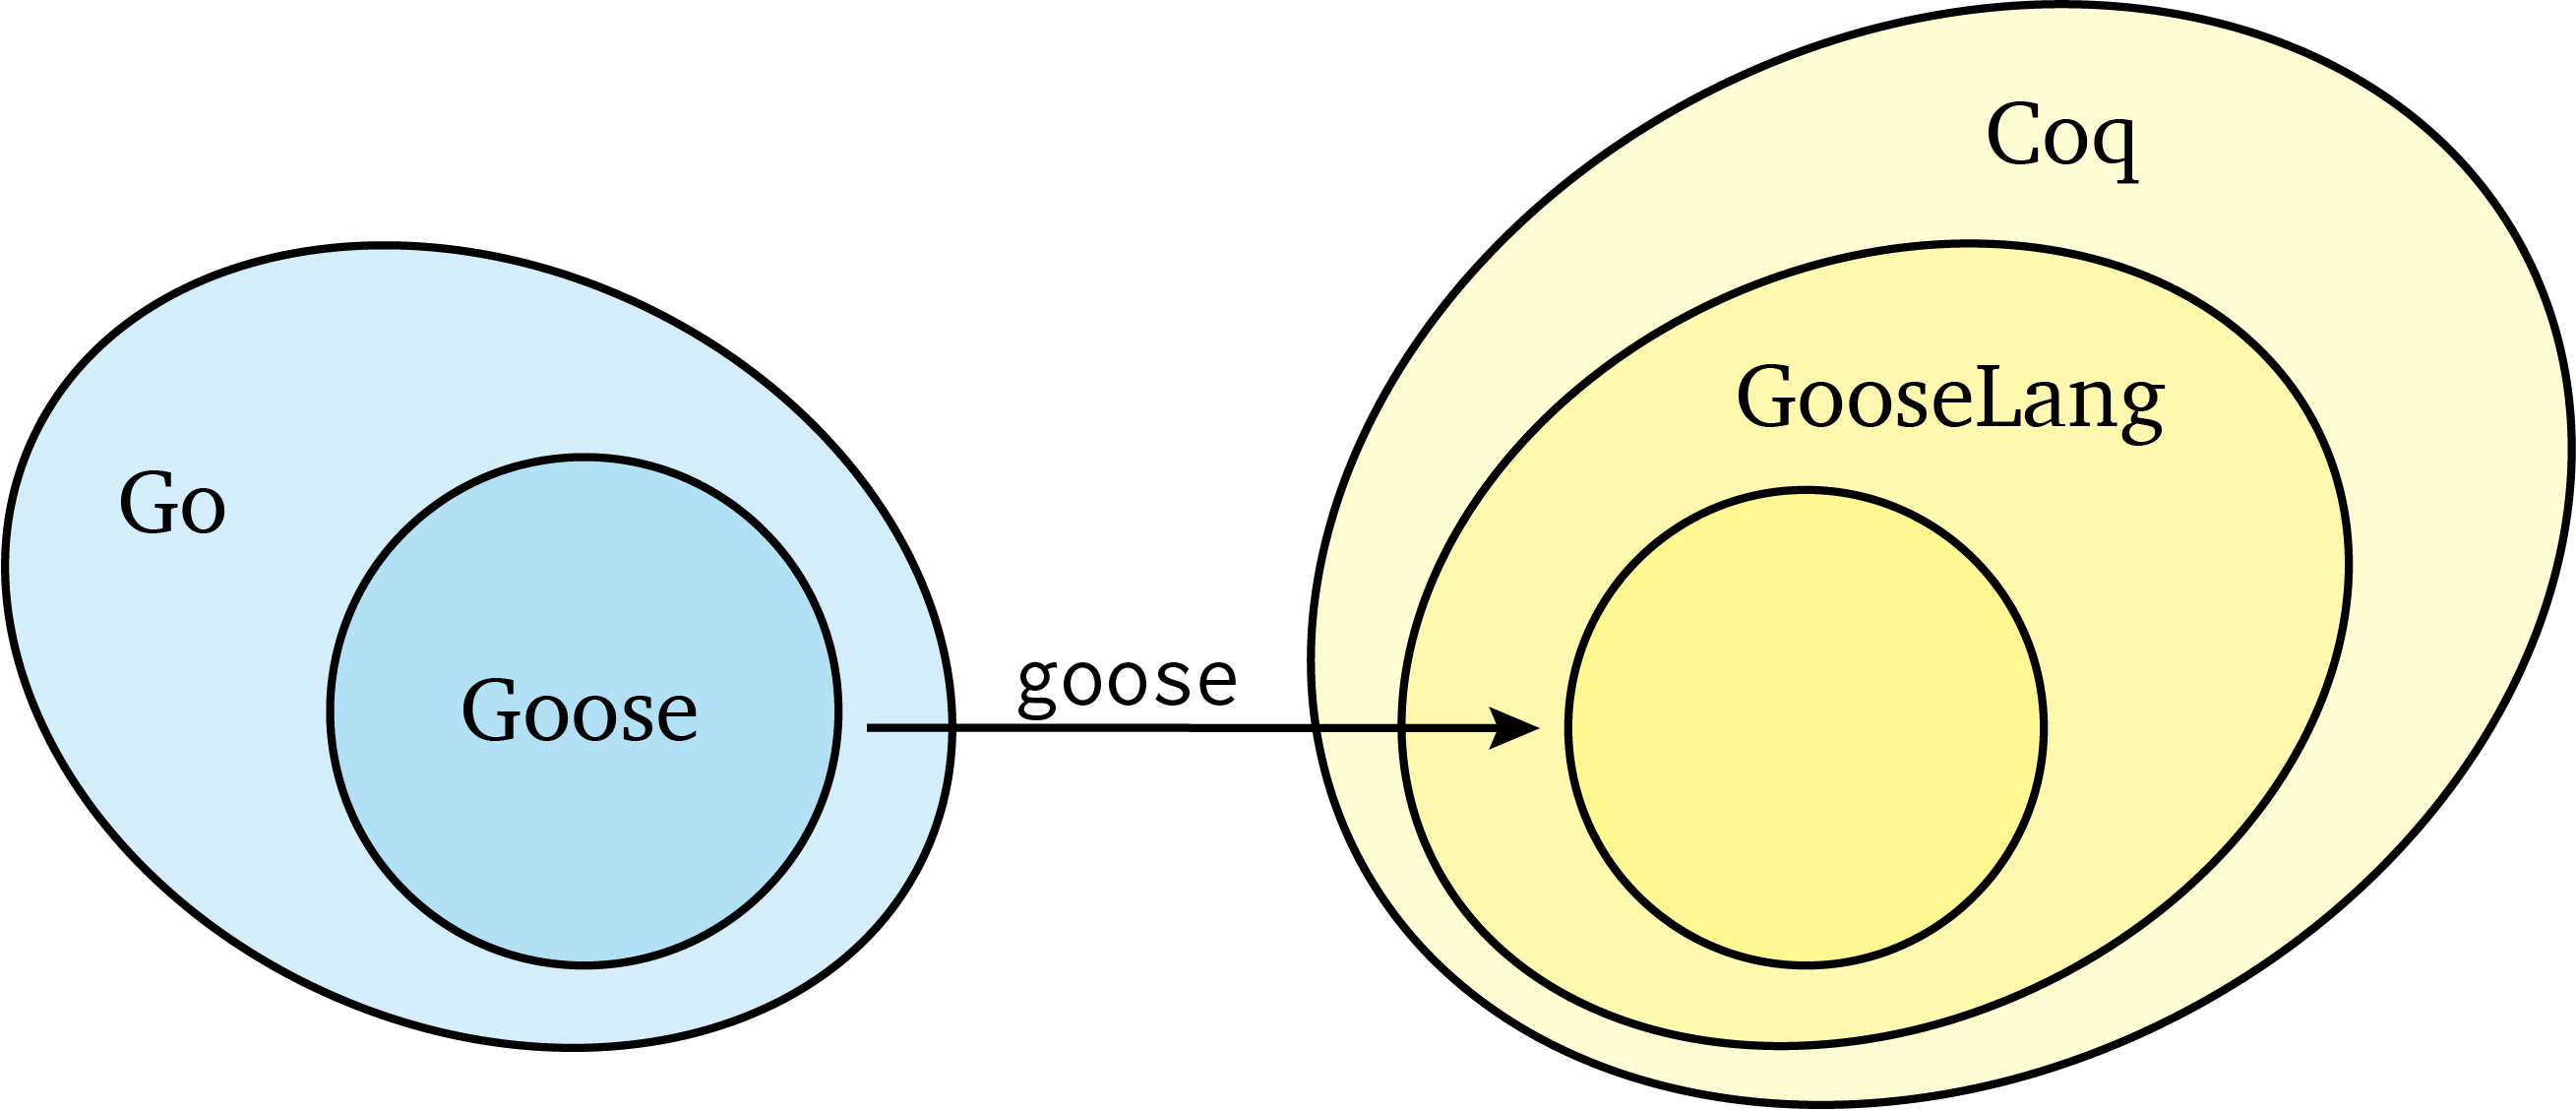
\includegraphics{fig/goose.png}
  \vspace{0.5\baselineskip}
  \caption[Representation of Goose's translation support]%
  {Pictorial representation of Goose's translation. Goose supports a subset of
    Go, which it translates to GooseLang. The target is more general, so not all
    of GooseLang can be produced from Go code. GooseLang itself is embedded in
    the Coq proof assistant.}
  \label{fig:goose:overview}
\end{figure}

An important aspect of GooseLang is supporting interactive proofs on top
of the translated code. The interactive proofs use separation logic, a
variant of Hoare logic, so specifications describe the behavior of each
individual function. In order to support verification of any translated
code, GooseLang comes with a specification for any primitive or function
that the translated code might refer to, including libraries like slices
used to model more sophisticated Go features. GooseLang has many
``pure'' operations that have no effect on the heap, due to many
primitive data types and operations (for example, there are both 8-,
32-, and 64-bit integers, and arithmetic and logical operations for
each). The specifications for these operations are handled with a single
lemma, which is applied automatically with a tactic \cc{wp_pures}.

Since our goal is to support interactive rather than automated proofs,
it is helpful to make the model simple to work with. The translation process maintains
a strong correspondence between the model and source code: each Go
package translates to a single Coq file, and each top-level declaration
in the Go code maps to a Gallina definition (a GooseLang constant or
function). Goose has a special case for translating immutable variables
to let bindings in GooseLang (rather than allocating a pointer that will
only be read). As a result, factoring out a sub-expression to a variable
has little impact on proofs.

The translation process sometimes translates a Go operation to a sophisticated
model in order to capture some corner-case behavior, for example in the model of
slices described in \cref{sec:goose:slices}. This complex models don't have an
undue affect on proofs as long as Goose's reasoning principles can abstract away
the complexity for common cases. The subsequent sections in this chapter
walk through several features of Go. Each section first describes a model that
implements the feature in GooseLang, which primarily aims to
be faithful to Go. Next, the section describes reasoning principles we developed for that
feature, in the form of separation logic assertions (for example, to
represent a slice) and Hoare triples (for example, to specify the
behavior of the \cc{append()} operation). The goal for the model is to capture
Go's behavior, whereas the reasoning
principles aim to make proofs using the model practical. See
\cref{fig:goose:workflow} for an overview of how
the code and proofs fit together when using Goose.

\begin{figure}
  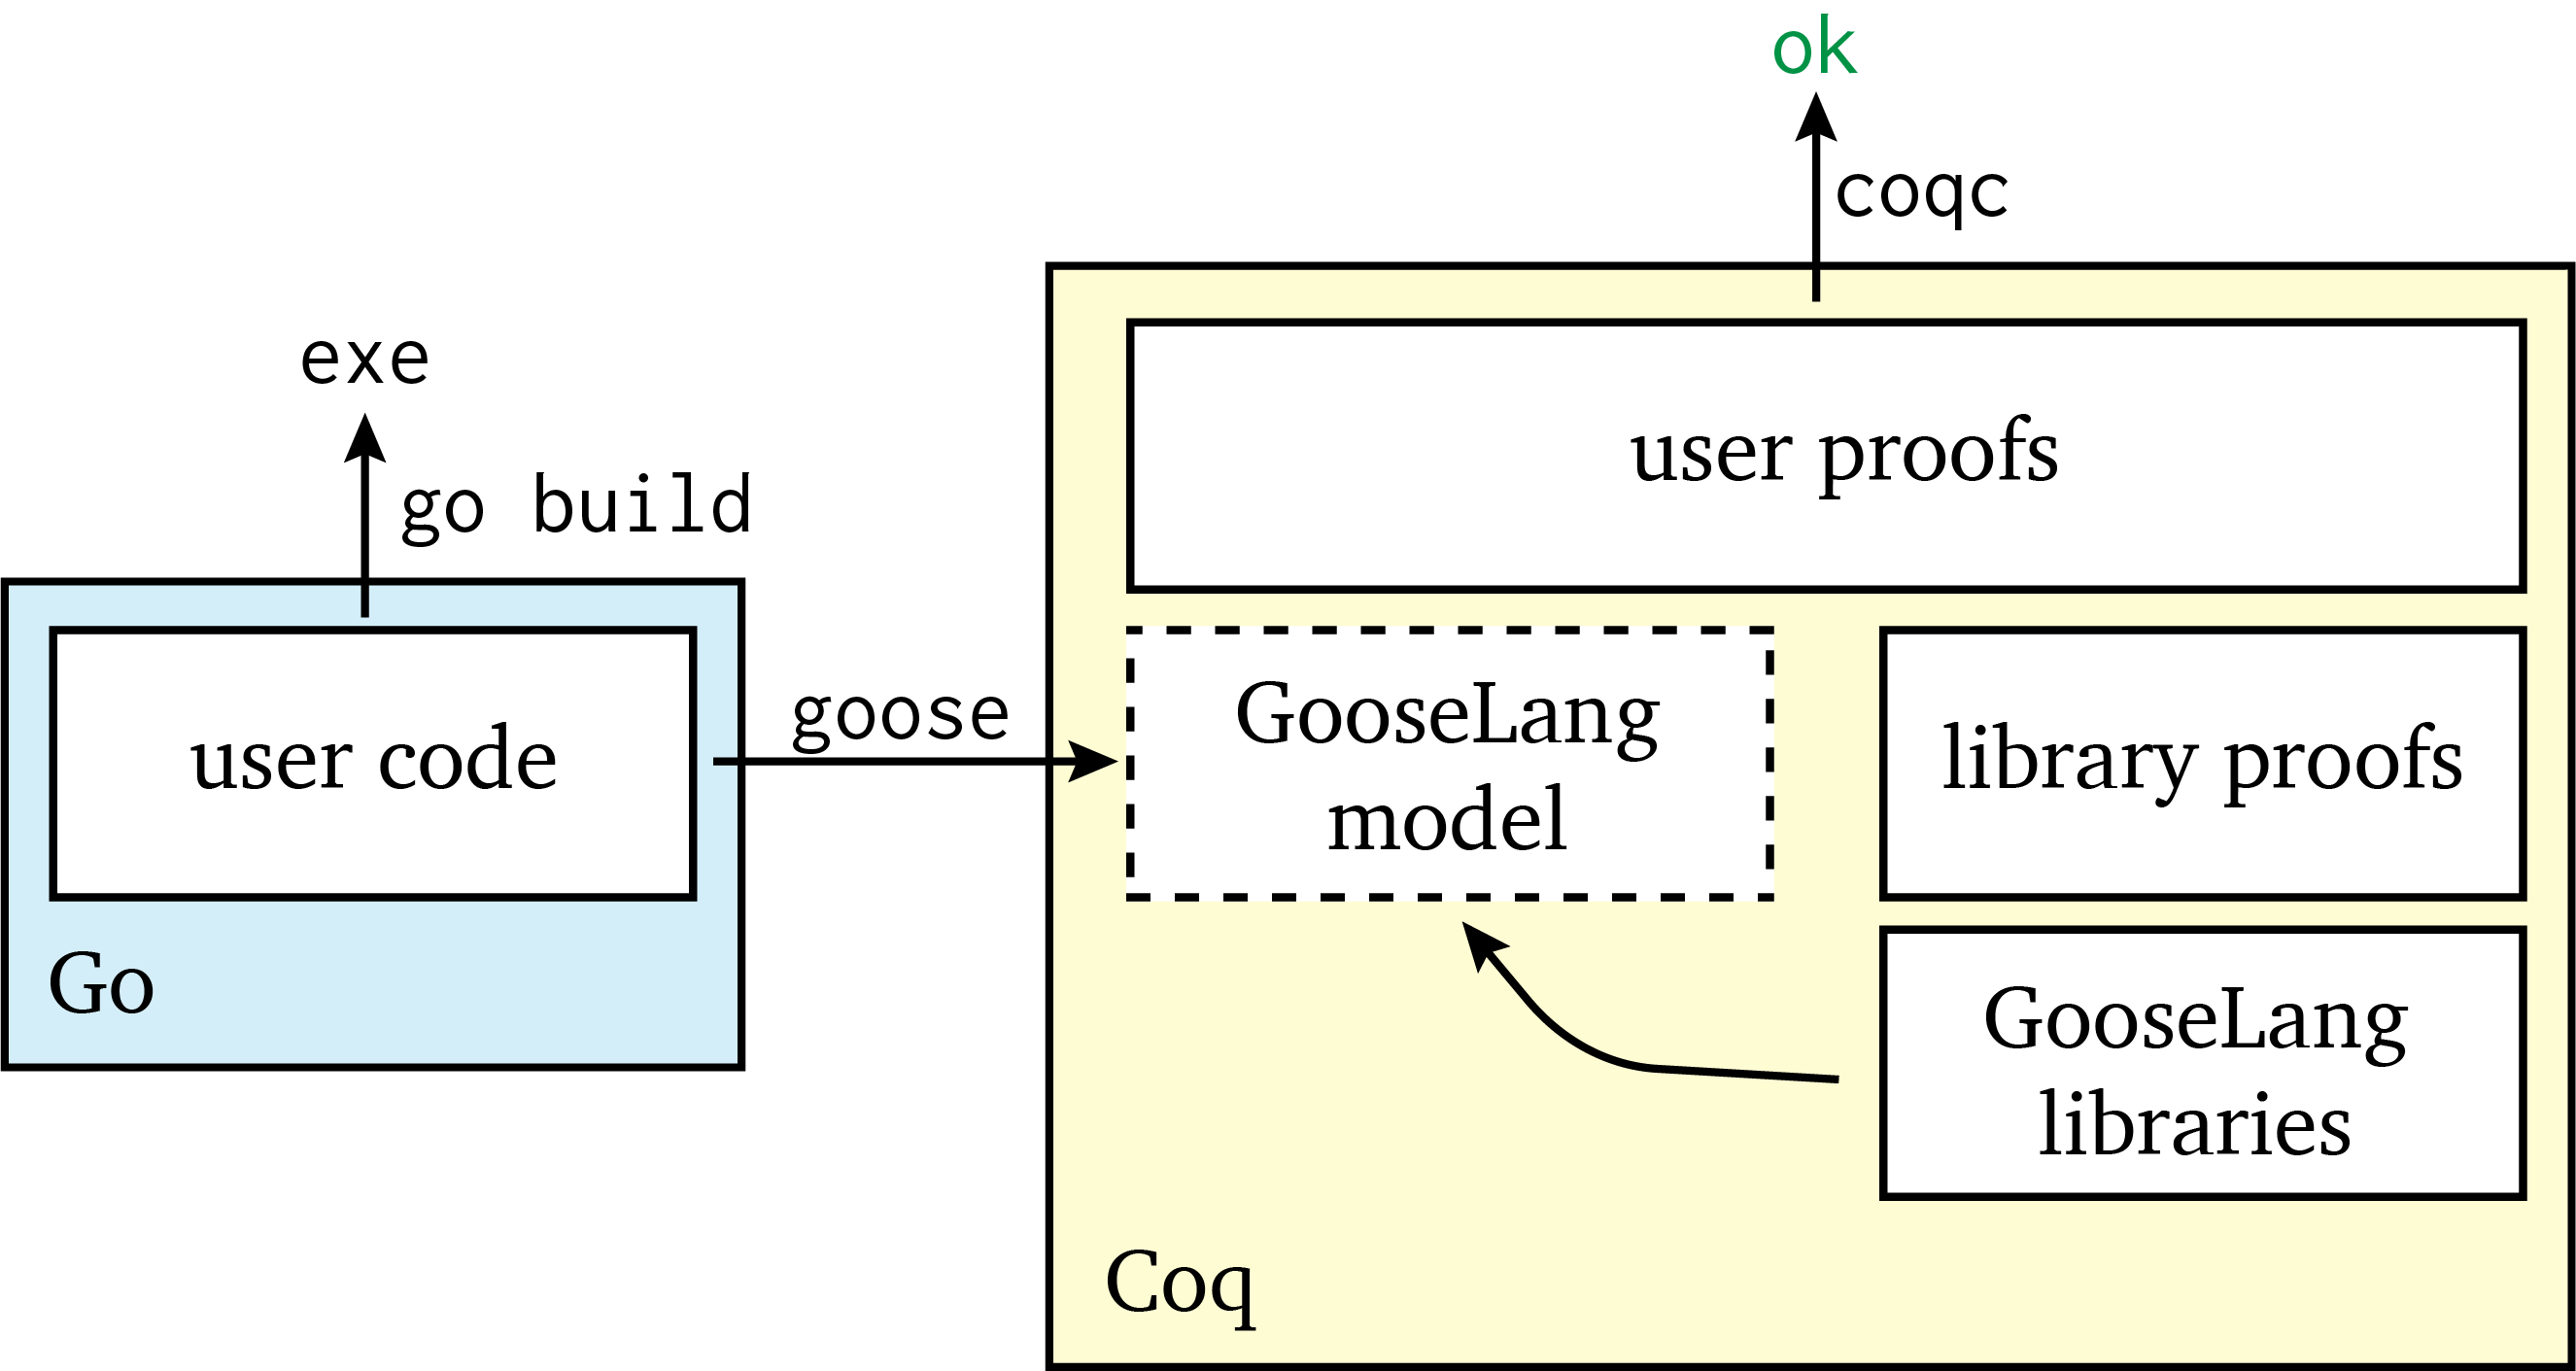
\includegraphics{fig/goose-proofs.png}
  \vspace{0.5\baselineskip}
  \caption[Workflow for verifying code with Goose]%
  {Workflow for verifying code using Goose. The user writes the code and
    proofs on top of the generated model. The model references libraries that
    model features of Go, which come equipped with proof libraries to make
    proofs easier. The code is ordinary Go that can be compiled, tested, and
    debugged with the usual Go tools. The proofs are all checked by the Coq
    proof assistant.}
  \label{fig:goose:workflow}
\end{figure}
